% 2.3.4.Solutions.tex
%	Last update: 2020/02/13 F.Kanehori
%newpage
\subsubsection{対処法}
\label{subsubsec:Solutions}
\parindent=0pt

前節で示した問題点への対処法について述べます。

\bigskip
\bf{ソースファイルの整合性}
\begin{narrow}[20pt]
	\SprLib のソースツリーにあるプロジェクトディレクトリ
	(Base, Collision, ...)を直接`\tt{add\_subdirectory}'すれば十分です。
\end{narrow}

\medskip
\bf{ビルドの最適性(無駄なコンパイル)}
\begin{narrow}[20pt]
	\SprLib, \it{App1, App2\,}などのすべてにおいて、
	ライブラリのオブジェクトが生成される場所を共通化してしまうことで
	この問題を回避することとします。
	具体的には、\SprLib ソースツリーの中(ビルドツリーの外)に
	オブジェクトの共通格納場所を作り、
	\SprLib およびすべてのアプリケーションで、
	ライブラリのオブジェクト格納ディレクトリをそこへのlinkとします。

	\begin{figure}[h]
	    \begin{center}
	    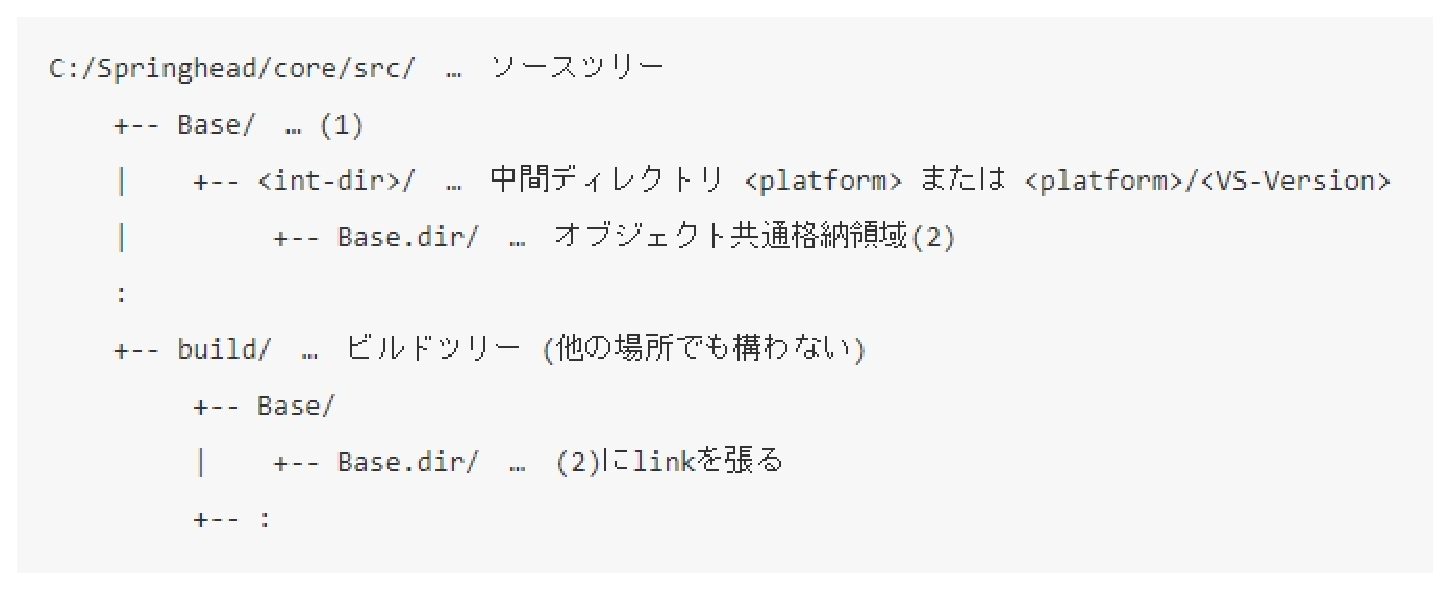
\includegraphics[width=1\textwidth]{fig/ApproachToBuildOptimization-1.eps}
	    \end{center}
	\end{figure}
	\Vskip{-.5\baselineskip}
	\begin{figure}[h]
	    \begin{center}
	    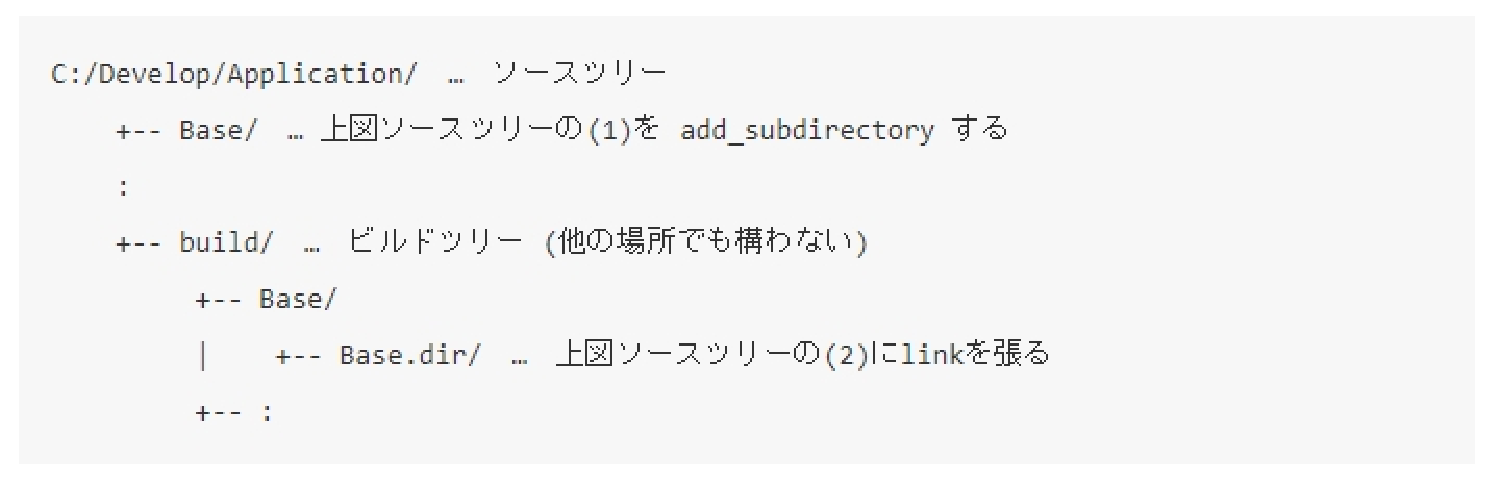
\includegraphics[width=1\textwidth]{fig/ApproachToBuildOptimization-2.eps}
	    \end{center}
	    \caption{ビルドの最適性への対処法}
	    \label{fig:ApproachToBuildOptimization}
	\end{figure}
%	\begin{figure}[h]
%    	\begin{narrow}[40pt]\begin{minipage}{\textwidth}
%		{\footnotesize{\dirtree{%
%			.1 \hspace{-10mm}C:/Springhead/core/src/ \Anno{ソースツリー}.
%			.2 Base/ \Anno{(1)}.
%			.3 <\it{int-dir\,}>/
%				\Anno{中間ディレクトリ <platform>
%					または<platform>/<VS-Version>}.
%			.4 Base.dir/ \Anno{オブジェクト共通格納領域(2)}.
%			.3 :.
%			.2 :.
%			.2 \BldDir \Anno{ビルドツリー (他の場所でも構わない)}.
%			.3 Base/.
%			.4 Base.dir/ \Anno{(2)にlinkを張る}.
%			.2 :.
%		}}}
%		\medskip
%    	\end{minipage}\end{narrow}
%    	\begin{narrow}[40pt]\begin{minipage}{\textwidth}
%		{\footnotesize{\dirtree{%
%			.1 \hspace{-10mm}C:/Develop/Application/ \Anno{ソースツリー}.
%			.2 Base/
%				\Anno{上図ソースツリーの(1)を\tt{add\_subdirectory}する}.
%			.2 :.
%			.2 \BldDir \Anno{ビルドツリー (他の場所でも構わない)}.
%			.3 Base/.
%			.4 Base.dir/ \Anno{上図ソースツリーの(2)にlinkを張る}.
%			.3 :.
%		}}}
%		\medskip
%  	\end{minipage}\end{narrow}
%	\caption{ビルドの最適性への対処法}
%	\label{fig:ApproachToBuildOptimization}
%	\end{figure}

	\medskip
	オブジェクトの共通格納領域を設定する作業は\SprLib の\cmake\ (configure)時に、
	linkを張る作業はアプリケーションの\cmake\ (configure)時に行なうものとします。
\end{narrow}

\medskip
\bf{プロジェクトファイルの整合性}
\begin{narrow}[20pt]
	ビルドの最適性の場合と同様、
	ソリューションファイルおよびプロジェクトファイルを共通化することで
	この問題に対処します。
	具体的には、\SprLib ビルドツリー上にあるものを最新の状態に保つことを前提として、
	すべてのアプリケーションについて、
	\SprLib のプロジェクトに関わるソリューションファイル
	およびプロジェクトファイルはすべて
	\SprLib ビルドツリーにあるものの複製をもつようにします。

	\medskip
	ただしこれでは不完全で、\App{1}で実施したプロジェクトファイルへの変更が
	\App{2}に伝わりません。
	このため\App{1}でプロジェクトファイルを変更した場合には、
	その変更を\SprLib ビルドツリーにあるプロジェクトファイルにコピーするものとします。
	つまり、\SprLib のビルドツリーにあるプロジェクトファイルを
	常に最新の状態に保つということです。

	\medskip
	この作業はアプリケーションのビルド時に行なうものとします。
	そのために、各アプリケーションのソリューションファイルに
	特別なターゲット`\tt{sync}'を作成し、
	このターゲットが毎回のビルドに先立って実行されるようにします。

	\begin{figure}[h]
	    \begin{center}
	    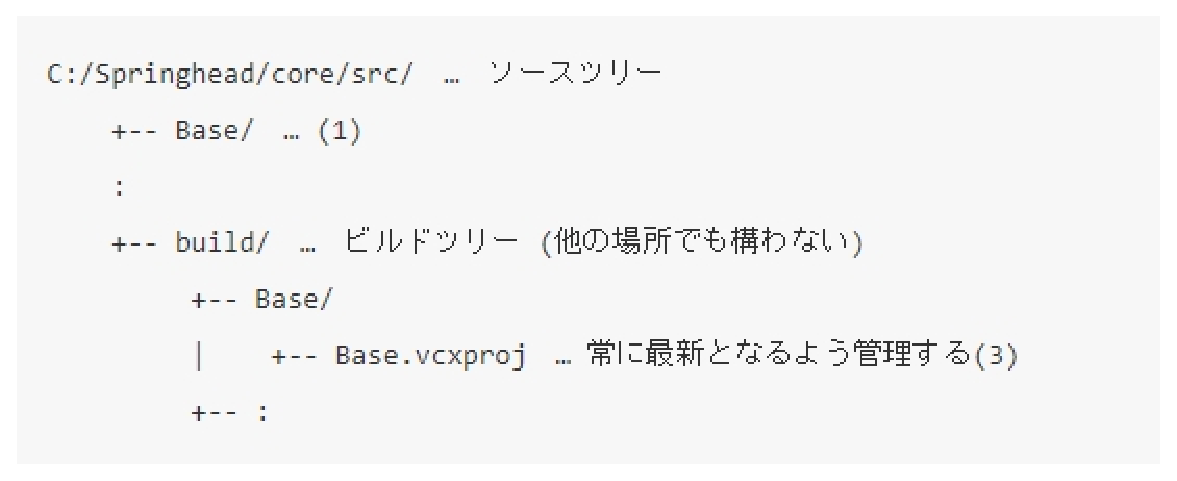
\includegraphics[width=.85\textwidth]{fig/ApproachToProjfileOptimization-1.eps}
	    \end{center}
	\end{figure}
	\Vskip{-.5\baselineskip}
	\begin{figure}[h]
	    \begin{center}
	    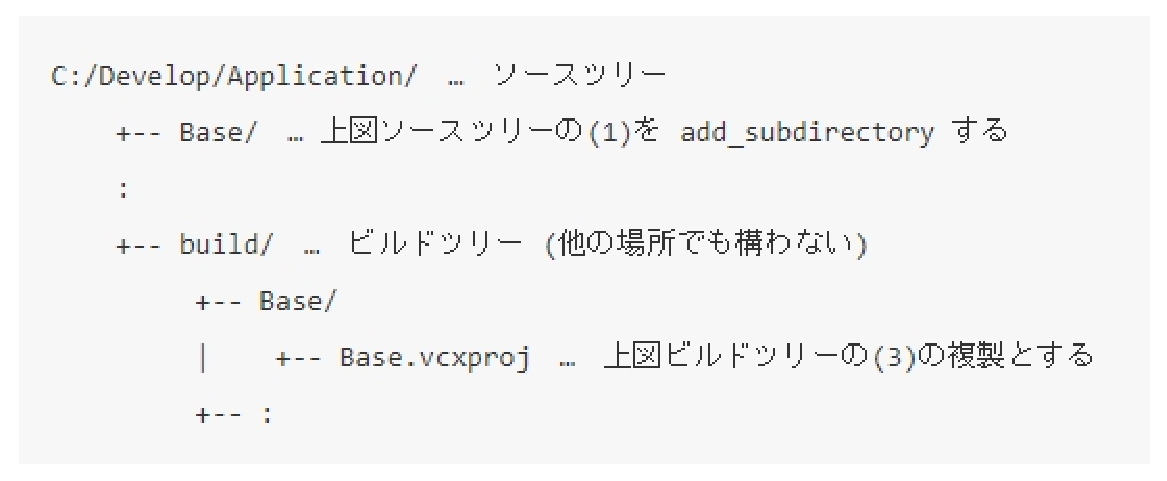
\includegraphics[width=.85\textwidth]{fig/ApproachToProjfileOptimization-2.eps}
	    \end{center}
	    \caption{プロジェクトファイルの最適性への対処法}
	    \label{fig:ApproachToProjfileOptimization}
	\end{figure}
%	\begin{figure}[h]
%    	\begin{narrow}[40pt]\begin{minipage}{\textwidth}
%		{\footnotesize{\dirtree{%
%			.1 \hspace{-10mm}C:/Springhead/core/src/ \Anno{ソースツリー}.
%			.2 Base/ \Anno{(1)}.
%			.2 :.
%			.2 \BldDir \Anno{ビルドツリー (他の場所でも構わない)}.
%			.3 Base/.
%			.4 Base.vcxproj \Anno{常に最新となるように管理する(3)}.
%			.2 :.
%		}}}
%		\medskip
%    	\end{minipage}\end{narrow}
%    	\begin{narrow}[40pt]\begin{minipage}{\textwidth}
%		{\footnotesize{\dirtree{%
%			.1 \hspace{-10mm}C:/Develop/Application/ \Anno{ソースツリー}.
%			.2 Base/ \Anno{上図ソースツリーの(1)を\tt{add\_subdirectory}する}.
%			.2 :.
%			.2 \BldDir \Anno{ビルドツリー (他の場所でも構わない)}.
%			.3 Base/.
%			.4 Base.vcxprj/ \Anno{上図ビルドツリーの(3)の複製とする}.
%			.3 :.
%		}}}
%		\medskip
%  	\end{minipage}\end{narrow}
%	\caption{プロジェクトファイルの最適性への対処法}
%	\label{fig:ApproachToProjfileOptimization}
%	\end{figure}
\end{narrow}

% end: 2.3.4.Solutions.tex
